\section{B-alberi}

I B-alberi sono \textbf{alberi bilanciati} adatti per memorizzare grandi masse di dati in memoria secondaria. Sono simili agli alberi rosso-neri, ma sono progettati per minimizzare gli accessi alla memoria secondaria. Le operazioni sono \textbf{insert}, \textbf{delete}, \textbf{search}, \textbf{split} e \textbf{join}.

I nodi dei B-alberi possono avere un numero di chiavi $n\ge 1$ ed $n+1$ figli.

\begin{figure}[htpd]
\centering
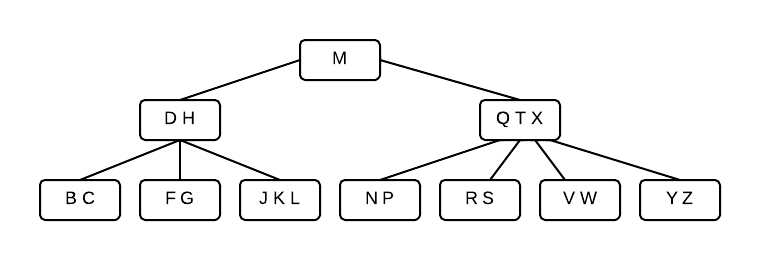
\includegraphics[width=100mm]{images/b-alberi1.png}
\end{figure}

\subsection{Definizione di un B-albero}

Un B-albero $T$ è un albero di radice $T.root$ tale che:

\begin{enumerate}

\item Ogni nodo $x$ contiene i seguenti campi:
	\begin{enumerate}
	\item $x.n$: il numero di chiavi presenti nel nodo;
	\item $x.key_1\le x.key_2 \le ... \le x.key_n $: le $x.n$ chiavi in ordine crescente;
	\item $x.leaf$: valore booleano che è true se il nodo $x$ è una foglia, false altrimenti.
	\end{enumerate}
\item Se il nodo non è una foglia contiene anche $x.c_1, X.c_2, x.c_{n+1}$: gli $n+1$ puntatori ai figli;
\item Le chiavi $x.key_1, x.key_2, ..., x.key_n$ di un nodo interno separano le chiavi dei sottoalberi. Se $k_i$ è una chiave qualsiasi del sottoalbero $x.c_i$, allora:

$$k_1 \le x.key_1 \le k_2 \le x.key_2 \le ... \le x.key_{x.n} \le k_{x.n+1}$$

\item Le foglie sono tutte alla stessa profondità $h$, detta \textbf{altezza dell'albero};
\item Vi sono limiti inferiori e superiori al numero di chiavi in un nodo, e tali limiti dipendono da una costante $t$ detta \textbf{grado minimo} del B-albero.
	\begin{enumerate}
	\item Ogni nodo, eccetto la radice, ha almeno $t-1$ chiavi e, se non è una foglia, ha almeno $t$ figli;
	\item Se l'albero non è vuoto la radice contiene almeno una chiave;
	\item Ogni nodo ha al più $2t-1$ chiavi e, se non è foglia, ha al più $2t$ figli.
	\end{enumerate}

\end{enumerate}

Ad ogni chiave sono generalmente associate delle informazioni ausiliarie. Assumeremo implicitamente che quando viene copiata una chiave vengono copiate anche tali informazioni. I B-alberi più semplici sono quelli con grado minimo $t=2$. Ogni nodo interno ha 2,3 o 4 figli.
Ogni albero non vuoto di grado minimo $t$ con $N$ chiavi ha altezza:

$$h \le \log_t\frac{N+1}{2}$$

\subsection{Operazioni sui B-alberi}

Adottiamo le seguenti convenzioni per le operazioni sui B-alberi:

\begin{enumerate}

\item La radice del B-albero è sempre in memoria;
\item I nodi passati come parametri alle procedure sono stati preventivamente caricati in memoria.

\end{enumerate}

\subsubsection{Creazione di un B-albero vuoto}

La procedura ausiliaria \textbf{ALLOCATE-NODE} alloca una pagina del disco da utilizzare come nuovo nodo nel tempo $O(1)$. Supponiamo che un nodo creato da ALLOCATE-NODE non richieda l'operazione DISK-WRITE.

\begin{lstlisting}[caption=Creazione di un B-albero]

B-TREE-CREATE(T)
	x = ALLOCATE-NODE()
	x.leaf = true
	x.n = 0
	DISK-WRITE(x)
	T.root = x

\end{lstlisting}

La procedura B-TREE-CREATE richiede $O(1)$ operazioni su disco e quindi un tempo di CPU pari a $O(1)$.

\subsubsection{Ricerca in un B-albero}

\begin{lstlisting}[mathescape=true, caption=Ricerca in un B-albero]

B-TREE-SEARCH(x, k)
	i = 1
	while i $\le$ x.n and k > $x.key_i$
		i = i+1
	if i$\le$ x.n and k == $x.key_i$
		return(x, i)
	elseif x.leaf
		return nil
	else DISK-READ(x,$c_i$)
		return B-TREE-SEARCH($x.c_i$, k)

\end{lstlisting}

La procedura richiede tempo $O(\log_2 N)$. Il numero di $DISK-READ$ è al più uguale all'altezza $h$ dell'albero, quindi $O(\log_tN)$. Il tempo di CPU della procedura è:

$$T\le(h+1)\log_2(2t-1)$$
$$=O(\log_tN\log_2t)$$
$$=O(\log_2N)$$

\subsubsection{Inserimento di una chiave}

L'aggiunta di  una chiave ad un B-albero può avvenire soltanto in una foglia e soltanto se la foglia non è piena, cioè non ha il numero massimo $2t-1$ di chiavi. Possiamo garantirci che la foglia a cui arriveremo non sia piena se ad ogni passo nella discesa dalla radice ci assicuriamo che il figlio su cui scendiamo non sia pieno. Nel caso in cui tale figlio sia pieno chiamiamo prima una particolare funzione \textbf{$SPLIT-CHILD$} che lo divide in due.

\begin{lstlisting}[mathescape=true, caption=Procedura di divisione di un nodo]

B-TREE-SPLIT-CHILD(x, i)
	z = ALLOCATE-NODE()
	y = $x.c_i$
	z.leaf = y.leaf
	z.n = t-1
	for j=1 to t-1
		$z.key_j$ = $y.key_{j+t}$
	if not y.leaf
		for j=1 to t
			$z.c_j$ = $y.c_{j+t}$
	y.n = t-1
	for j=x.n+1 downto i+1
		$x.c_{j+1}$ = $x.c_j$
	$x.c_{i+1}=z$
	for j=x.n downto i
		$x.key_{j+1}=x.key_j$
	$x.key_i=y.key_t$
	x.n = x.n+1
	DISK-WRITE(y)
	DISK-WRITE(z)
	DISK-WRITE(x)

\end{lstlisting}

Inseriamo ora una chiave $k$ nel B-albero $T$ di altezza $h$ con un singolo passaggio in discesa nell'albero, richiedendo $O(h)$ accessi. Il tempo di CPU richiesto è $O(th)=O(t\log_tn)$. La procedura B-TRSERT usa B-TREE-SPLIT-CHILD per garantire che la ricorsione non arrivi mai a un nodo pieno.

\begin{lstlisting}[mathescape=true, caption=Inserimento di una chiave]

B-TREE-INSERT(T,k)
	r = T.root
	if r.n == 2t-1
		s = ALLOCATE-NODE()
		T.root = s
		s.leaf = false
		s.n = =
		s.$c_1$ = r
		B-TREE-SPLIT-CHILD(s,1)
		B-TREE-INSERT-NONFULL(s,k)
	else
		B-TREE-INSERT-NONFULL(r,k)

\end{lstlisting}

La procedura finisce chiamando B-TREE-INSERT-NONFULL per inserire la chiave $k$ nell'albero che ha un nodo radice non pieno. La procedura B-TREE-INSERT-NONFULL effettua la ricorsione quante volte serve per discendere l'albero, assicurandosi che il nodo in cui effettua la ricorsione non sia mai pieno, chiamando B-TREE-SPLIT-CHILD se necessario.

\begin{lstlisting}[mathescape=true, caption=B-Tree insert nonfull]

B-TREE-INSERT-NONFULL(x,k)
	i = x.n
	if x.leaf
		while $i\ge 1$ and k<$x.key_i$
			x.$key_{i+1}$ = x.$key_i$
			i = i-1
		x.$key_{i+1}$=k
		x.n = x.n+1
		DISK-WRITE(x)
	else while $i\ge 1$ and k<x.$key_i$
			i = i-1
		i = i+1
		DISK-READ(x.$c_i$)
		if $x.c_i$.n == 2t-1
			B-TREE-SPLIT-CHILD(x,i)
			if k>$x.key_i$
				i = i+1
			B-TREE-INSERT-NONFULL(x.$c_i$,k)

\end{lstlisting}

Il tempo totale della CPU è $O(th)=O(t\log_tn)$.

\subsubsection{Cancellazione di una chiave}

La cancellazione di una chiave da un B-albero è analoga all'inserimento, ma un po' più complicata, perchè una chiave può essere cancellata da un nodo qualsiasi e l'eliminazione di una chiave da un nodo interno richiede che i figli del nodo vengano riorganizzati. Azichè lo pseudocodice, descriveremo il funzionamento dell'operazione di cancellazione.

\begin{enumerate}

\item Se la chiave si trova nel nodo $x$ e $x$ è una foglia, cancellare la chiave $k$ da $x$;
\item Se la chiave $k$ si trova nel nodo $x$ e $x$ è un nodo interno, eseguire le seguenti operazioni:
	\begin{enumerate}
	\item Se il figlio $y$ che precede $k$ nel nodo $x$ ha almeno $t$ chiavi, trovare il predecessore $k'$ di $k$ nel sottoalbero con radice in $y$. Cancellare ricorsivamente $k'$ e sostituire $k$ con $k'$ in $x$;
	\item Simmetricamente, se il figlio $z$ che segue $k$ nel nodo $x$ ha almeno $t$ chiavi, trovare il successore $k'$ di $k$ nel sottoalbero con radice in $z$. Cancellare ricorsivamente $k'$ e sostituire $k$ con $k'$ in $x$;
	\item Altrimenti, se entrambi i nodi $y$ e $z$ hanno soltanto $t-1$ chiavi, fondere $k$ e tutto $z$ nel nodo $y$, in modo che $x$ perda sia $k$ sia il puntatore a $z$; adesso $y$ contiene $2t-1$ chiavi. Poi, rilasciare $z$ e cancellare ricorsivamente $k$ da $y$.
	\end{enumerate}
\item Se la chiave $k$  non è presente nel nodo interno $x$, determinare la radice $x.c_i$ del sottoalbero appropriato che deve contenere $k$, se $k$ è davvero presente nell'albero. Se $x.c_i$ ha soltanto $t-1$ chiavi, eseguire il passo 3a o 3b, se necessario, per avere la garanzia di arrivare a un nodo che contiene almeno $t$ chiavi. Poi, finire effettuando la ricorsione sul figlio appropriato di $x$.
	\begin{enumerate}
	\item Se $x.c_i$ ha soltanto $t-1$ chiavi, ma ha un fratello adiacente con almeno $t$ chiavi, assegnare a $x.c_i$ una chiave extra, spostando in basso una chiave da $x$ in $x.c_i$, spostando in alto una chiave dal fratello sinistro o destro di $x.c_i$ in $x$ e, infine, spostando in $x.c_i$ un puntatore al figlio del fratello (quello adiacente alla chiave spostata);
	\item Se $x.c_i$ ed entrambi i fratelli adiacenti di $x.c_i$ hanno $t-1$ chiavi, fondere $x.c_i$ con un fratello in un nuovo nodo; questo richiede che una chiave venga spostata in basso da $x$ nel nuovo nodo per diventare la chiave mediana di questo nodo.
	\end{enumerate}
\end{enumerate}